\documentclass[tikz,border=0.1cm]{standalone}
\usepackage{tikz}
\usetikzlibrary{bayesnet}
\usepackage{amsmath, amsfonts, amssymb}
\tikzset{>=latex}

\begin{document}
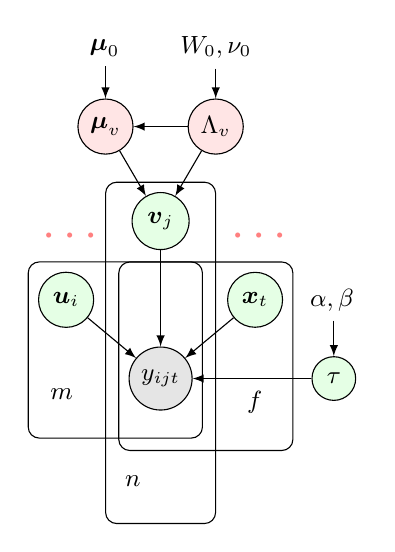
\begin{tikzpicture}
\node[circle,draw=black,fill=gray!20,inner sep=0pt,minimum size=0.8cm] (obs) at (2,-1) {\small{$y_{ijt}$}};
\node[circle,draw=black,fill=green!10] (ui) at (0.8,0) {\small{$\boldsymbol{u}_{i}$}};
\node[circle,draw=black,fill=green!10] (vj) at (2,1) {\small{$\boldsymbol{v}_{j}$}};
\node[circle,draw=black,fill=green!10] (xt) at (3.2,0) {\small{$\boldsymbol{x}_{t}$}};
\node[circle,draw=black,fill=green!10] (tau) at (4.2,-1) {\small{$\tau$}};
\path[draw=black,->] (ui) edge (obs);
\path[draw=black,->] (vj) edge (obs);
\path[draw=black,->] (xt) edge (obs);
\path[draw=black,->] (tau) edge (obs);
\node [text width=0.8cm] (m) at (1,-1.2) {\small{$m$}};
\plate[] {plate1} {(obs)(ui)(m)} { };
\node [text width=0.9cm] (n) at (2,-2.3) {\small{$n$}};
\plate[] {plate2} {(obs)(vj)(n)} { };
\node [text width=0.2cm] (f) at (3.2,-1.3) {\small{$f$}};
\plate[] {plate3} {(obs)(xt)(f)} { };
\node[circle,draw=black,fill=red!10,inner sep=0pt,minimum size=0.7cm] (muv) at (1.3,2.2) {\small{$\boldsymbol{\mu}_{v}$}};
\node[circle,draw=black,fill=red!10,inner sep=0pt,minimum size=0.7cm] (lambdav) at (2.7,2.2) {\small{$\Lambda_{v}$}};
\node[text width=0.6cm] (gamma) at (4.2,0) {\small{$\alpha,\beta$}};
\node[text width=0.4cm] (mu0) at (1.3,3.2) {\small{$\boldsymbol{\mu}_{0}$}};
\node[text width=0.9cm] (wnu0) at (2.7,3.2) {\small{$W_{0},\nu_{0}$}};
\node[text width=0.6cm] (cdots1) at (0.8,0.8) {\LARGE\color{red!50}{$\cdots$}};
\node[text width=0.6cm] (cdots2) at (3.2,0.8) {\LARGE\color{red!50}{$\cdots$}};
\path[draw=black,->] (muv) edge (vj);
\path[draw=black,->] (lambdav) edge (vj);
\path[draw=black,->] (lambdav) edge (muv);
\path[draw=black,->] (mu0) edge (muv);
\path[draw=black,->] (wnu0) edge (lambdav);
\path[draw=black,->] (gamma) edge (tau);
\end{tikzpicture}
\end{document}